% Author: Santiago Faci <santiago.faci@gmail.com>
% http://github.com/sfaci/masc

\documentclass[xcolor={dvipsnames}]{beamer}
\setbeamertemplate{navigation symbols}{}

\usepackage{beamerthemeshadow}
\usepackage[spanish]{babel}
\usepackage{url}
\usepackage[utf8]{inputenc}

\definecolor{resalta}{cmyk}{0,1,0,0}

\usepackage{listings}
\lstset{basicstyle=\tiny\ttfamily,breaklines=true}
\lstset{framextopmargin=50pt}
\lstset{keywordstyle=\tiny\color{blue}\bfseries}
\lstset{stringstyle=\tiny\color{red}\ttfamily}
\lstset{commentstyle=\tiny\color{OliveGreen}\ttfamily}
\lstset{showstringspaces=false}

\begin{document}
\title{masc: malware (web) scanner}  
\author{Santiago Faci\\ \url{sfaci@fundacionmontessori.com}}
\institute{\small{Colegio Montessori (Zaragoza)}}
\date{\Large{Hackathon Cybercamp 2017}} 

% logo
\titlegraphic{
\includegraphics[scale=0.2]{cybercamp}
}

\begin{frame}
\titlepage
\end{frame}

\begin{frame}\frametitle{Índice}\tableofcontents
\end{frame} 


\section{¿Qué iba a ser masc?} 
\begin{frame}\frametitle{¿Qué iba a ser masc?} 

    \begin{block}{malware web scanner}
    Escanea un sitio web ya comprometido en busca de malware con el objetivo de eliminarlo
    \end{block}

    \begin{itemize}
        \item Busca y/o limpia, automáticamente, malware en un sitio web que sabemos que ha sido atacado
        \item Aunque no pensemos que hemos sido atacados, podemos ejecutarlo periodicamente para comprobarlo. No todos los ataques son ruidosos
        \item Comportamiento a medida de algunos CMS concretos
        \item Trabaja basándose en diccionarios que pueden ser ampliados y mejorados
        \item La idea es que sea fácilmente extensible para que se adapte a otros CMS y arquitecturas web
    \end{itemize}
\end{frame}

\section{Propuestas para el Hackathon}
\subsection{¿Qué quería hacer yo?}
\begin{frame}\frametitle{Propuestas para el hackathon}
    \begin{block}{Mis ideas}
    \begin{itemize}
        \item Hacer que \emph{masc} trabaje con diferentes CMS (Drupal, Joomla, Magento, . . .)
        \item Convertirlo también en una aplicación web (con ayuda de Django)
        \item Crear una arquitectura que lo haga facilmente extensible
        \item Comprobar los permisos de los ficheros y directorios
        \item Ofrecer al usuario la posibilidad de restaurar el funcionamiento del sitio web
        \item Utilizar las firmas del proyecto \emph{WebMalwareScanner} de \emph{OWASP}
    \end{itemize}
    \end{block}
\end{frame}

\subsection{Nuevas propuestas}
\begin{frame}\frametitle{Aportaciones del jurado del Hackathon}
    \begin{block}{Nuevas ideas}
    \begin{itemize}
        \item Registrar toda la actividad de la herramienta por medio de ficheros log
        \item Dar la opción al usuario de realizar una limpieza que permita añadir cierta protección al sitio
        \item Dar opción al usuario para que pueda restaurar su sitio en el estado previo al paso de la herramienta
        \item Siempre que la herramienta realice una limpieza, que almacene un backup previo
        \item Añadir una opción para hacer un backup directamente
        \item Y algunas issues
    \end{itemize}
    \end{block}
\end{frame}

\section{¿Qué es masc ahora?} 
\begin{frame}\frametitle{¿Qué es masc ahora?} 

    \begin{block}{malware web scanner}
    Escanea un sitio web ya comprometido en busca de malware con el objetivo de eliminarlo
    \end{block}

    \begin{itemize}
        \item Busca y/o limpia, automáticamente, malware en un sitio web que sabemos que ha sido atacado
        \item Comportamiento a medida de algunos CMS concretos (Actualmente muy centrado en WordPress)
        \item Utiliza instalaciones limpias para comparar y encontrar ficheros sospechosos
        \item Trabaja principalmente basándose en firmas y reglas YARA del proyecto OWASP WebMalwareScanner
        \item Fácil de extender para añadir soporte específico para otros CMS
    \end{itemize}
\end{frame}

\begin{frame}\frametitle{¿Qué es masc ahora?}
    \begin{itemize}
        \item Antes de realizar una limpieza del malware del sitio realiza un backup del mismo
        \item El usuario puede restaurar ese backup previo usando la herramienta
        \item Toda la actividad de \emph{masc} queda registrada en logs
        \item Además limpia contenido no necesario del sitio y ejecuta algunas otras operaciones para ayudar en su protección
            \begin{itemize}
                \item Elimina todo tipo de README del core y temas de WordPress
                \item Evita el listado de directorios
                \item Elimina el metatag que identifica la versión de WordPress
                \item Corrige los permisos
            \end{itemize}
        \item Monitoriza el sitio web completo en busca de cambios y los registra en un log
    \end{itemize}
\end{frame}

\section{Demo}
\subsection{La herramienta}
\begin{frame}\frametitle{masc como herramienta}
    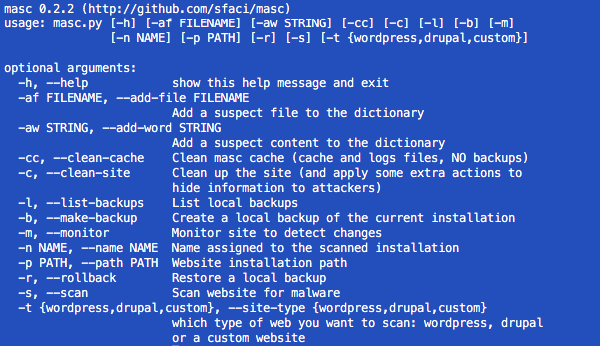
\includegraphics[scale=0.35]{options} 
\end{frame}

\subsection{Ecaneo de un sitio}
\begin{frame}\frametitle{Escaneo de un sitio 'custom'}
    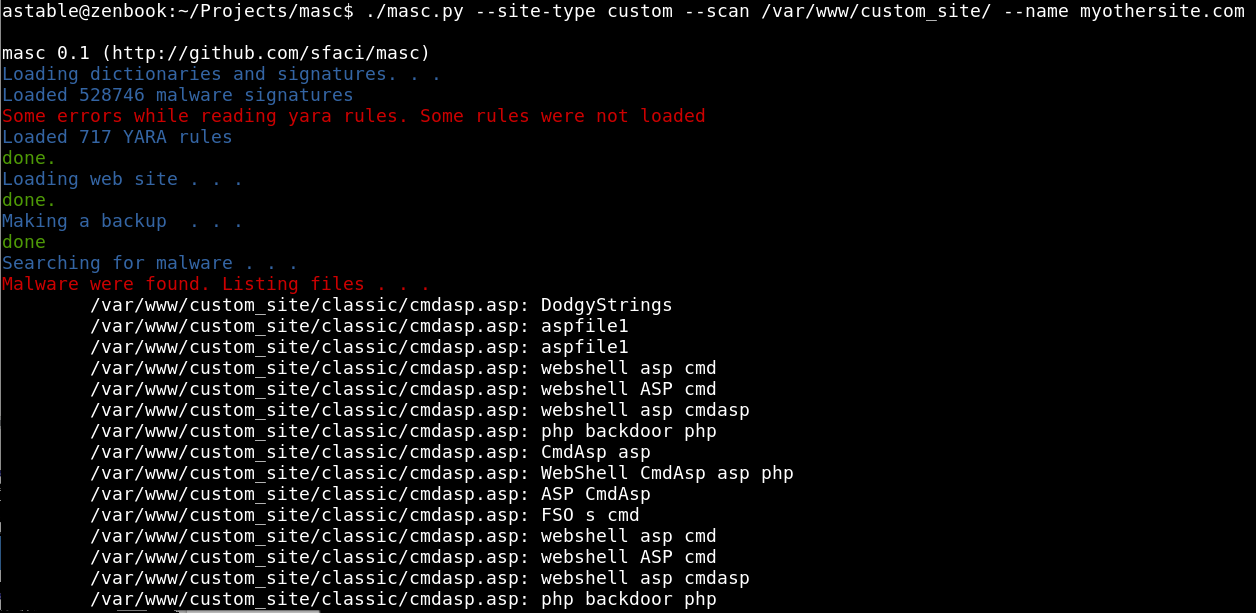
\includegraphics[scale=0.25]{custom_scan} 
\end{frame}

\subsection{Escaneo y limpieza de un sitio}
\begin{frame}\frametitle{Escaneo y limpieza de un sitio WordPress}
    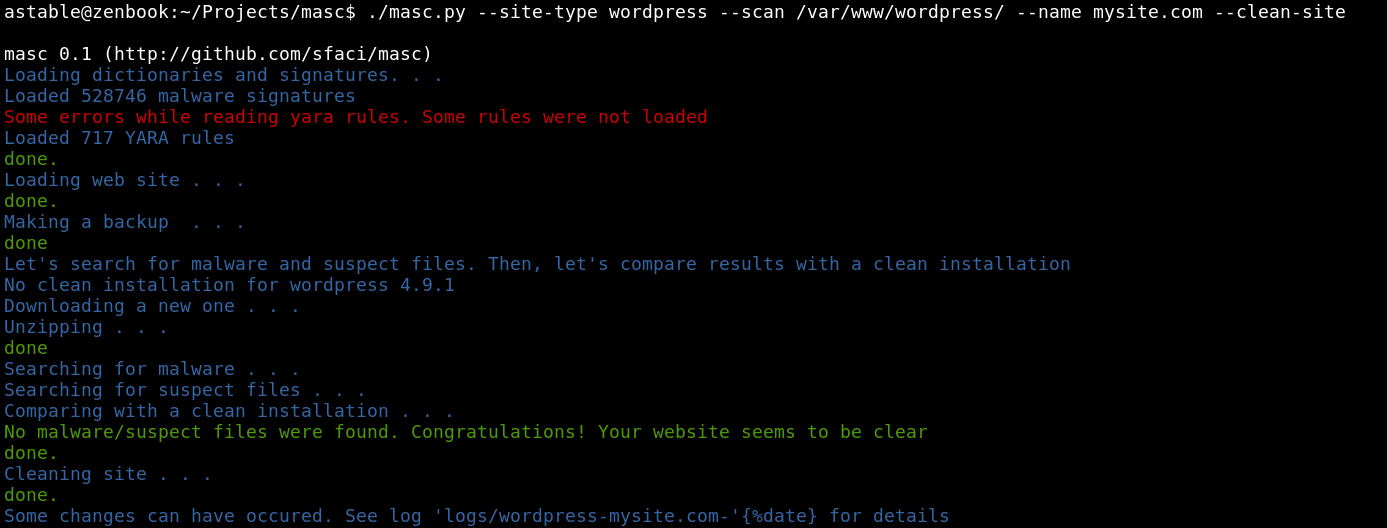
\includegraphics[scale=0.21]{complete} 
\end{frame}

\subsection{Rollback}
\begin{frame}\frametitle{Rollback}
    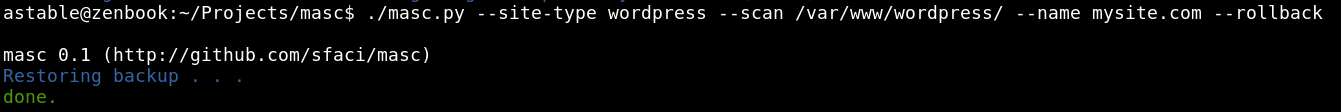
\includegraphics[scale=0.23]{rollback} 
\end{frame}

\subsection{Backups}
\begin{frame}\frametitle{Lista de backups}
    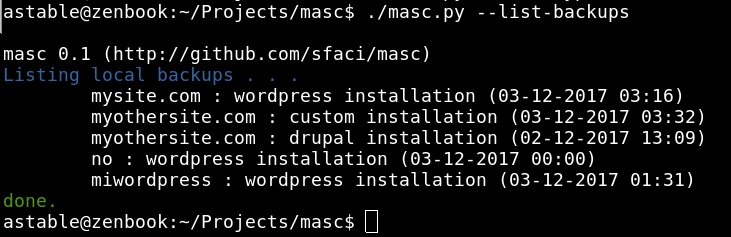
\includegraphics[scale=0.4]{list-backups} 
\end{frame}

\subsection{Logs}
\begin{frame}\frametitle{Ficheros log}
    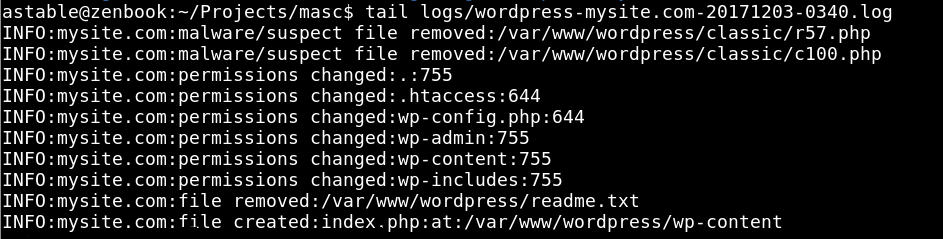
\includegraphics[scale=0.3]{log} 
\end{frame}

\section{Ideas para el futuro}
\begin{frame}\frametitle{Ideas para el futuro}
    \begin{block}{Cómo puede crecer masc}
    \begin{itemize}
        \item Ampliar la base de datos de firmas y reglas YARA
        \item Que sea capaz de limpiar código inyectado en ficheros legítimos
        \item Diseñar un interfaz web
        \item Escaneo remoto de sitios web
        \item Convertirlo en herramienta web como servicio en la nube
    \end{itemize}
    \end{block}
\end{frame}

\begin{frame}\frametitle{Fin}
    \begin{center}
        
\includegraphics[scale=0.3]{cybercamp} 
     \end{center}
      \begin{center}
        \huge{Hackathon CyberCamp 2017} 
     \end{center}
\end{frame}

\end{document}
